\documentclass[border=12pt]{standalone}
\usepackage[utf8]{inputenc}
\usepackage[utf8]{vietnam}
\usepackage{amsmath,amsfonts,amssymb}
\usepackage{siunitx}
\usepackage{tikz}
\usetikzlibrary{arrows, decorations.markings, calc, fadings, decorations.pathreplacing, patterns, decorations.pathmorphing, positioning}
\begin{document}
	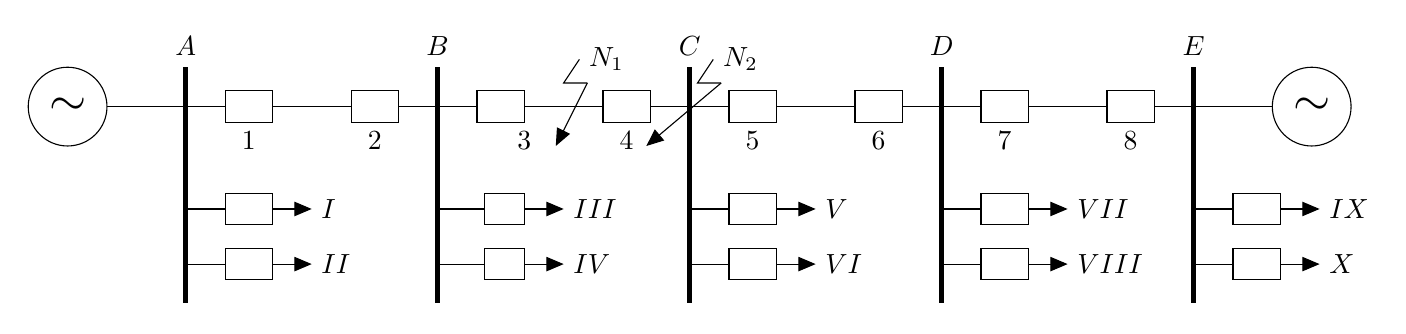
\begin{tikzpicture}[>=triangle 45]
		\draw (0,0) circle (.5)  node{\LARGE{$\mathbf{\sim}$}};
		\draw (0.5, 0) -- (1.5,0);
		\draw[ultra thick] (1.5,0.5) node[above]{$A$} -- (1.5, -2.5);
		\draw (1.5, 0) -- (2, 0); \draw (2,0.2) rectangle (2.6,-0.2); \draw (2.3,-.2) node[below]{$1$}; \draw (2.6, 0) -- (3.6,0);\draw (3.6,0.2) rectangle (4.2,-0.2); \draw (3.9,-.2) node[below]{$2$}; \draw (4.2,0) -- (4.7,0);
		\draw (1.5, -1.3) -- (2,-1.3); \draw (2,-1.1) rectangle (2.6,-1.5); \draw[->] (2.6,-1.3) -- (3.1,-1.3) node[right]{$I$};
		\draw (1.5, -2) -- (2,-2); \draw (2,-1.8) rectangle (2.6,-2.2); \draw[->] (2.6,-2) -- (3.1,-2) node[right]{$II$};
					
		\draw[ultra thick] (4.7,0.5) node[above]{$B$} -- (4.7, -2.5);
		\draw (4.7, 0) -- (5.2, 0); \draw (5.2,0.2) rectangle (5.8,-0.2); \draw (5.8,-.2) node[below]{$3$}; \draw (5.8, 0) -- (6.8,0);\draw (6.8,0.2) rectangle (7.4,-0.2); \draw (7.1,-.2) node[below]{$4$}; \draw (7.4,0) -- (7.9,0); \draw (6.5,0.6) node[right]{$N_1$} -- (6.3,0.3) -- (6.6,0.3); \draw[->] (6.6,0.3) -- (6.2,-.5);
		\draw (4.7, -1.3) -- (5.3,-1.3); \draw (5.3,-1.1) rectangle (5.8,-1.5); \draw[->] (5.8,-1.3) -- (6.3,-1.3) node[right]{$III$};
		\draw (4.7, -2) -- (5.3,-2); \draw (5.3,-1.8) rectangle (5.8,-2.2); \draw[->] (5.8,-2) -- (6.3,-2) node[right]{$IV$};
					
		\draw[ultra thick] (7.9,0.5) node[above]{$C$} -- (7.9, -2.5); 
		\draw (7.9, 0) -- (8.4, 0); \draw (8.4,0.2) rectangle (9,-0.2); \draw (8.7,-.2) node[below]{$5$}; \draw (9, 0) -- (10,0);\draw (10,0.2) rectangle (10.6,-0.2); \draw (10.3,-.2) node[below]{$6$}; \draw (10.6,0) -- (11.1,0);  \draw (8.2,0.6) node[right]{$N_2$} -- (8,0.3) -- (8.3,0.3); \draw[->] (8.3,0.3) -- (7.35,-.5);
		\draw (7.9, -1.3) -- (8.4,-1.3); \draw (8.4,-1.1) rectangle (9,-1.5); \draw[->] (9,-1.3) -- (9.5,-1.3) node[right]{$V$};
		\draw (7.9, -2) -- (8.4,-2); \draw (8.4,-1.8) rectangle (9,-2.2); \draw[->] (9,-2) -- (9.5,-2) node[right]{$VI$};
					
		\draw[ultra thick] (11.1,0.5) node[above]{$D$} -- (11.1, -2.5);
		\draw (11.1, 0) -- (11.6, 0); \draw (11.6,0.2) rectangle (12.2,-0.2); \draw (11.9,-.2) node[below]{$7$}; \draw (12.2, 0) -- (13.2,0);\draw (13.2,0.2) rectangle (13.8,-0.2); \draw (13.5,-.2) node[below]{$8$}; \draw (13.8,0) -- (14.3,0);
		\draw (11.1, -1.3) -- (11.6,-1.3); \draw (11.6,-1.1) rectangle (12.2,-1.5); \draw[->] (12.2,-1.3) -- (12.7,-1.3) node[right]{$VII$};
		\draw (11.1, -2) -- (11.6,-2); \draw (11.6,-1.8) rectangle (12.2,-2.2); \draw[->] (12.2,-2) -- (12.7,-2) node[right]{$VIII$};
					
		\draw[ultra thick] (14.3,0.5) node[above]{$E$} -- (14.3, -2.5);
		\draw (14.3, 0) -- (15.3, 0); \draw (15.8,0) circle (.5)  node{\LARGE{$\mathbf{\sim}$}};
		\draw (14.3, -1.3) -- (14.8,-1.3); \draw (14.8,-1.1) rectangle (15.4,-1.5); \draw[->] (15.4,-1.3) -- (15.9,-1.3) node[right]{$IX$};
		\draw (14.3, -2) -- (14.8,-2); \draw (14.8,-1.8) rectangle (15.4,-2.2); \draw[->] (15.4,-2) -- (15.9,-2) node[right]{$X$};
	\end{tikzpicture}
\end{document} 